69. \begin{figure}[ht!]
\center{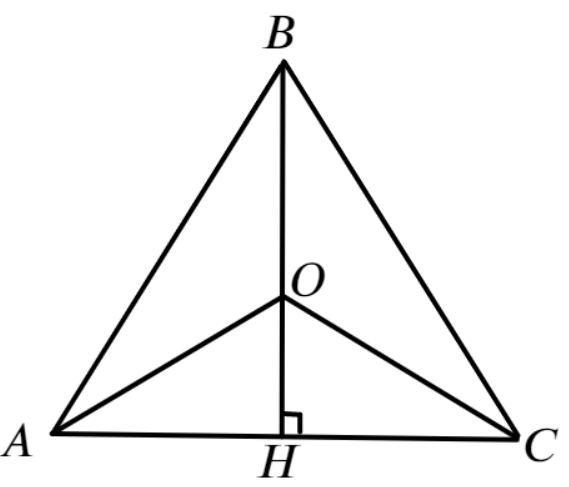
\includegraphics[scale=0.35]{g9-69.png}}
\end{figure}\\
Проведём из вершины высоту $BH$ и отметим на ней центр описанной окружности $O$ (высота является серединным перпендикуляром, поэтому он ей принадлежит). Тогда $OH=BH-BO=8-5=3,\ HC=\sqrt{5^2-3^2}=4,\ AC=2HC=8,\ S_{\Delta ABC}=\cfrac{1}{2}\cdot8\cdot8=32\text{ см}^2.$\\
